% 原书 p.63–p.70（PDF p.71–p.78）
\section{$J$-全纯曲线（第二部分）（$J$-Holomorphic Curve, Part Two）}

\begin{keytakeaways}
\begin{itemize}
  \item 几何图像：辛化 $SM=\R\times M$ 上的 $J$-全纯曲线，由于 $M\to\R$ 的
        $r$-分量是次调和函数，不可能像闭曲面那样存在，必须定义在带刺点的
        Riemann 曲面上；其「端」沿 $s\to\pm\infty$ 收敛到闭 Reeb 轨道。
  \item 数学工具：与 $\dd(\ee^r\alpha)$ 相容的 $J$（沿 $r$ 不变、交换
        $\partial_r$ 与 $R_\alpha$、在 $\xi$ 上取 $\dd\alpha$-相容结构）、
        (3.19)–(3.20) 的局部方程、Hofer 能量 $E_{\mathrm{Hofer}}$。
  \item 本节结论：Hofer 能量把平凡柱面从无穷能量「重整化」为有限值
        （命题 3.3.1、定理 3.3.1）；闭 Reeb 轨道由此实现为 $J$-全纯曲线的
        渐近端，但要证明这种曲线的存在仍是最困难的核心问题。
\end{itemize}
\end{keytakeaways}

% >>> p071
研究辛流形的有力工具是 $J$-全纯曲线理论（见 §1.4）。由于维数上的原因，
给定切触流形 $(M,\xi)$ 时，并不显然存在一套直接适用于 $(M,\xi)$ 的曲线理论。
然而，借助定义 3.2.1 中的辛化 $SM$，可以尝试研究 $SM$ 中的 $J$-全纯曲线。
回忆：对 $\omega$-相容的殆复结构 $J$，可微映射 $u:(\Sigma,j)\to(X,\omega,J)$
称为 $J$-\textbf{全纯的}，若 $J\circ\dd u=\dd u\circ j$（见定义 1.4.1）。
当 $X=SM$ 时，有若干自然的问题。

\textbf{问题 1}：如何在辛化 $SM$ 上选取殆复结构 $J$，使 $J$ 与
$\dd(\ee^r\alpha)$ 相容？

\textbf{问题 2}：由于 $SM$ 是非紧流形，从几何上看，$SM$ 中的 $J$-全纯曲线
是什么样子？

\textbf{问题 3}：回忆 $J$-全纯曲线 $u$ 的能量定义为
$E(u):=\int_\Sigma u^*\omega$（见 (1.9)）。在 $SM$ 的情形，$u$ 的能量会呈现
怎样的行为？

我们将在本节余下部分回答这些问题。

给定任意切触流形 $(M,\xi=\ker\alpha)$，我们在 $SM$ 上选取殆复结构 $J$，
使其满足以下条件：
\begin{enumerate}[label=(\roman*)]
  \item $J$ 沿 $r$ 方向不变（回忆 $r$ 是 $SM$ 的 $\R$ 分量坐标），即
        $J_{(r,x)}=J_{r+c,x}$ 对任意 $c\in\R$ 与 $(r,x)\in SM$ 成立；
  \item $J(\partial_r)=R_\alpha$，$J(R_\alpha)=-\partial_r$，其中 $R_\alpha$
        是 $(M,\xi=\ker\alpha)$ 的 Reeb 向量场；
  \item 限制 $J|_\xi$ 是超平面场 $\xi$ 上的殆复结构，且
        $\dd\alpha|_\xi(\cdot,J\cdot)$ 在 $\xi$ 上定义黎曼度量（记为 $g$）。
\end{enumerate}
这样的殆复结构 $J$ 与 $\dd(\ee^r\alpha)$ 相容，这回答了上面的问题 1。例如，
对 $v,w\in\xi$，有
\begin{align*}
  \ee^r(\dd r\wedge\alpha+\dd\alpha)(Jv,Jw)
  &=\ee^r g(Jv,w)
   =\ee^r g(w,Jv)\\
  &=\ee^r\dd\alpha(w,-v)
   =\ee^r(\dd r\wedge\alpha+\dd\alpha)(v,w).
\end{align*}
同时，对 $v\in\xi$，有
$\dd(\ee^r\alpha)(v,Jv)=\ee^r\dd\alpha(v,Jv)=\ee^r g(v,v)>0$。再举一例，
当 $v=\partial_r$、$w=R_\alpha$ 时，有
$\ee^r(\dd r\wedge\alpha+\dd\alpha)(\partial_r,R_\alpha)
=\ee^r(1+0)=\ee^r>0$。其余情形可同理验证。

对上面的问题 2，按定义 1.4.1，考虑 $(\Sigma,j)$ 上的标准局部坐标 $(s,t)$，
其中 $\Sigma$ 上的复结构 $j$ 满足 $j\partial_t=-\partial_s$。
% >>> p072
在这些坐标下，$J$-全纯条件等价于
\begin{equation}\tag{3.17}
  J(u(s,t))\frac{\partial u}{\partial t}(s,t)
  +\frac{\partial u}{\partial s}(s,t)=0 .
\end{equation}
由于 $SM$ 有两个分量，即 $M$ 分量与 $\R$ 分量，我们把 $u$ 写成
$u(s,t)=(u_M(s,t),u_\R(s,t))$，于是偏微分方程 (3.17) 可改写为
\begin{equation}\tag{3.18}
  J(u(s,t))\Bigl(\frac{\partial u_\R}{\partial t},
  \frac{\partial u_M}{\partial t}\Bigr)
  +\Bigl(\frac{\partial u_\R}{\partial s},
  \frac{\partial u_M}{\partial s}\Bigr)=0 .
\end{equation}
由于 $(M,\xi=\ker\alpha)$ 是切触流形，其切空间局部地自然分裂为切触超平面
$\xi$ 与由 $R_\alpha$ 生成的 Reeb 方向。记 $\pi_\xi:TM\to\xi$ 为到
$\xi$-分量的投影，则可把方程 (3.18) 进一步拆分为
\begin{align*}
  &J(u(s,t))\Bigl(\frac{\partial u_\R}{\partial t},
  \alpha\Bigl(\frac{\partial u_M}{\partial t}\Bigr),
  \pi_\xi\Bigl(\frac{\partial u_M}{\partial t}\Bigr)\Bigr)\\
  &\qquad+\Bigl(\frac{\partial u_\R}{\partial s},
  \alpha\Bigl(\frac{\partial u_M}{\partial s}\Bigr),
  \pi_\xi\Bigl(\frac{\partial u_M}{\partial s}\Bigr)\Bigr)=0,
\end{align*}
其中 $R_\alpha$-分量直接由对 $\alpha$ 的求值给出。于是，由此处 $J$ 的定义
性质——特别是它交换 $\partial_r$ 与 $R_\alpha$——可得
\begin{equation}\tag{3.19}
  J(u(s,t))\frac{\partial u_\R}{\partial t}
  =\alpha\Bigl(\frac{\partial u_M}{\partial s}\Bigr),
  \quad\text{即}\quad
  \frac{\partial u_\R}{\partial t}
  =-\alpha\Bigl(\frac{\partial u_M}{\partial s}\Bigr).
\end{equation}
类似地，有
\begin{equation}\tag{3.20}
  \frac{\partial u_\R}{\partial s}
  =\alpha\Bigl(\frac{\partial u_M}{\partial t}\Bigr),
  \quad\text{且}\quad
  J(u(s,t))\pi_\xi\Bigl(\frac{\partial u_M}{\partial t}\Bigr)
  +\pi_\xi\Bigl(\frac{\partial u_M}{\partial s}\Bigr)=0 .
\end{equation}

% [Tutor Note: 原文疑误——(3.19) 中第一个等号与紧随其后的「即」在符号上不相容：
% 由 $J(\partial_r)=R_\alpha$ 可知 $J(u)\frac{\partial u_\R}{\partial t}$ 是
% $R_\alpha$ 方向的向量，再对 $\alpha$ 求值应得
% $\frac{\partial u_\R}{\partial t}$ 本身；而正确的关系式是
% $\frac{\partial u_\R}{\partial t}=-\alpha(\frac{\partial u_M}{\partial s})$
% （这正是 (3.18) 的 $R_\alpha$-分量，即 $J$ 交换 $\partial_r$ 与 $R_\alpha$
% 并取负号的结果）。建议把第一个等号读作「$J(u)\frac{\partial u_\R}{\partial t}
% +\alpha(\frac{\partial u_M}{\partial s})R_\alpha=0$」。已记入
% review_ch03.md。]

现在断言：$\R$ 分量 $u_\R:(\Sigma,j)\to\R$ 是次调和函数。换言之，Laplace
算子 $\Delta u_\R$ 局部非负。为看出这点，按 Laplace 算子的定义，
\begin{align*}
  \Delta u_\R
  &=\frac{\partial}{\partial s}\Bigl(\frac{\partial u_\R}{\partial s}\Bigr)
   +\frac{\partial}{\partial t}\Bigl(\frac{\partial u_\R}{\partial t}\Bigr)\\
  &=\frac{\partial}{\partial s}\alpha\Bigl(
   \frac{\partial u_M}{\partial t}\Bigr)
   -\frac{\partial}{\partial t}\alpha\Bigl(
   \frac{\partial u_M}{\partial s}\Bigr)\\
  &=\frac{\partial}{\partial s}(u_M^*\alpha)\Bigl(\frac{\partial}{\partial t}\Bigr)
   -\frac{\partial}{\partial t}(u_M^*\alpha)\Bigl(\frac{\partial}{\partial s}\Bigr)\\
  &=\dd(u_M^*\alpha)\Bigl(\frac{\partial}{\partial s},
   \frac{\partial}{\partial t}\Bigr)
   =\dd\alpha\Bigl(\frac{\partial u_M}{\partial s},
   \frac{\partial u_M}{\partial t}\Bigr).
\end{align*}
由于 $\dd\alpha$ 在 $R_\alpha$ 分量上恒为零，投影到超平面场 $\xi$ 便得
% >>> p073
\begin{align*}
  \dd\alpha\Bigl(\pi_\xi\Bigl(\frac{\partial u_M}{\partial s}\Bigr),
  \pi_\xi\Bigl(\frac{\partial u_M}{\partial t}\Bigr)\Bigr)
  &=\dd\alpha\Bigl(-J\pi_\xi\Bigl(\frac{\partial u_M}{\partial t}\Bigr),
  \pi_\xi\Bigl(\frac{\partial u_M}{\partial t}\Bigr)\Bigr)\\
  &=g\Bigl(\pi_\xi\Bigl(\frac{\partial u_M}{\partial t}\Bigr),
  \pi_\xi\Bigl(\frac{\partial u_M}{\partial t}\Bigr)\Bigr)\ge0,
\end{align*}
其中最后一个等号来自 (3.20)。

回忆非定常次调和函数的一个重要性质：它\textbf{不}容许任何局部最大值。假设
我们处于 §1.4 中的同一设定，即区域 $(\Sigma,j)$ 是闭 Riemann 曲面，则得到
矛盾：$\operatorname{im}(u_\R)$ 是 $\R$ 的紧子集，必取得最大值（除非
$u_\R$ 为常数）。因此，为避免这一矛盾，需要以某种方式修改曲面 $\Sigma$。
一种办法是考虑\textbf{带刺点的 Riemann 曲面}（punctured Riemann surface）：
\[
  \dot\Sigma:=\Sigma\setminus\Gamma
  =\Sigma\setminus\{p_1,\dots,p_n\},
\]
其中 $\Gamma=\{p_1,\dots,p_n\}$ 是 $\Sigma$ 中有限个点的集合（见图 3.5）。

\begin{figure}[htbp]
  \centering
  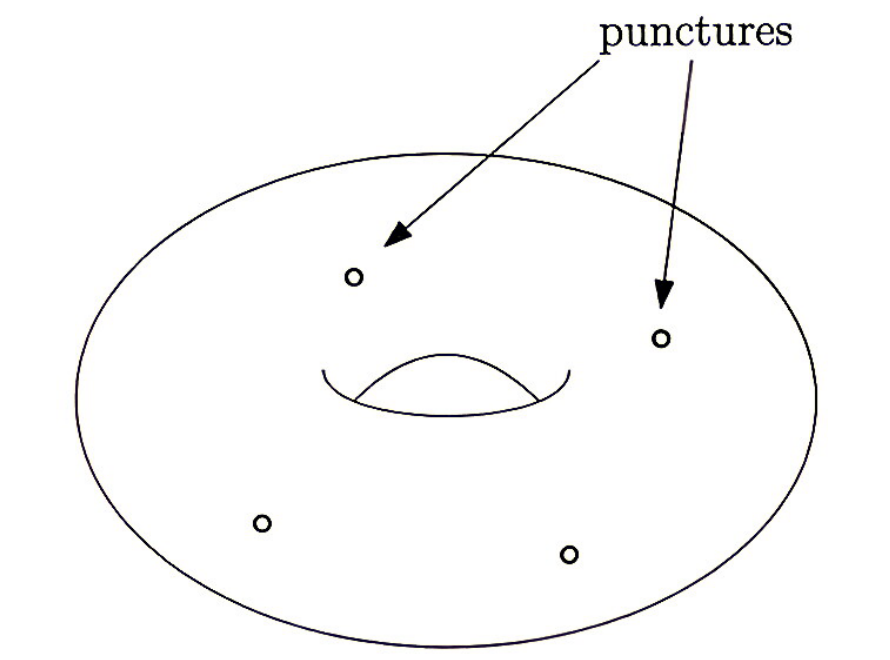
\includegraphics[width=0.52\linewidth]{figures/fig_p073_1.png}
  \caption*{图 3.5\quad 带刺点的环面 $\dot\Sigma_{g=1}$
  （原书 p.65, Figure 3.5）}
\end{figure}

在每个刺点 $p\in\Gamma$ 附近局部地看，它像一个带刺点的圆盘
$D\setminus\{0\}$。带刺点的圆盘双全纯于\textbf{正半柱面}
$[0,\infty)\times S^1$ 或\textbf{负半柱面}
$(-\infty,0]\times S^1$。在坐标
$(s,t)\in[0,\infty)\times S^1$ 或 $(s,t)\in(-\infty,0]\times S^1$ 中
（$s$ 为 $\R$ 分量，$t$ 为 $S^1$ 分量），双全纯映射可显式给出如下：
\begin{equation}\tag{3.21}
  (s,t)\mapsto\ee^{-2\pi(s+\sqrt{-1}t)}\in D\setminus\{0\},
  \quad\text{或}\quad
  (s,t)\mapsto\ee^{2\pi(s+\sqrt{-1}t)}\in D\setminus\{0\},
\end{equation}
分别对应这两种情形。从几何上看，映射 (3.21) 把刺点附近的邻域拉长成一根
长「管」（见图 3.6）。

% >>> p074
\begin{figure}[htbp]
  \centering
  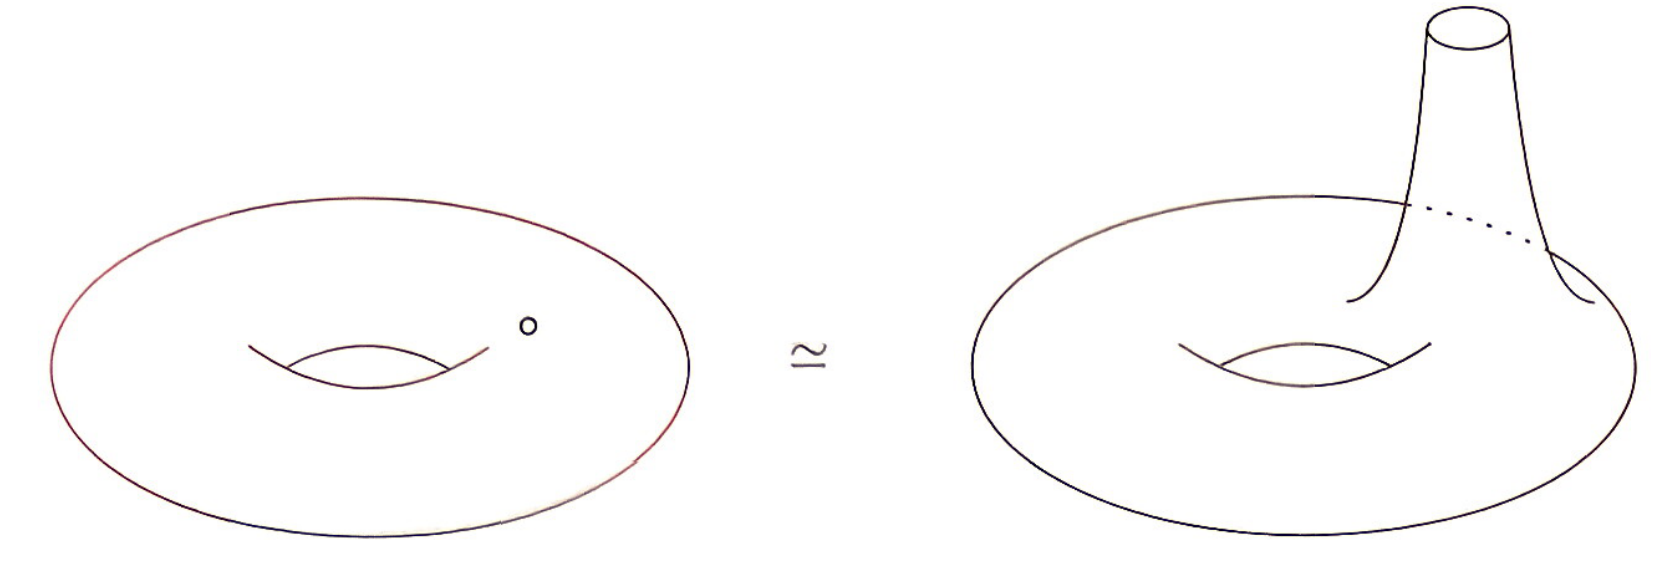
\includegraphics[width=0.85\linewidth]{figures/fig_p074_1.png}
  \caption*{图 3.6\quad 环面 $\dot\Sigma_{g=1}$ 上刺点附近的「管状」邻域
  （原书 p.66, Figure 3.6）}
\end{figure}

\begin{wexam}{3.3.1}
考虑带刺点的球面 $\dot\Sigma_{g=0}=S^2\setminus\Gamma$。当 $\#\Gamma$
变化时，这些区域可以与一些有众所周知名称的区域等同起来，如图 3.7 所示。
\begin{itemize}
  \item 当 $\#\Gamma=1$ 时，曲线
        $u:(\dot\Sigma_{g=0},j)\to(M,\omega,J)$ 称为
        \textbf{$J$-全纯平面}（$J$-holomorphic plane）。
  \item 当 $\#\Gamma=2$ 时，曲线
        $u:(\dot\Sigma_{g=0},j)\to(M,\omega,J)$ 称为
        \textbf{$J$-全纯柱面}（$J$-holomorphic cylinder）。
  \item 当 $\#\Gamma=3$ 时，曲线
        $u:(\dot\Sigma_{g=0},j)\to(M,\omega,J)$ 称为
        \textbf{裤子}（pair-of-pants）。
\end{itemize}
上述每一类曲线在发现各种辛刚性时都起着重要作用（我们将在后面的章节中看到
其中一些）。\hfill$//$
\end{wexam}

% [Tutor Note: 记号提示——此处以及例 3.3.2、§3.3 末尾出现的 $(M,\omega,J)$
% 沿用 §1.4 中「一般辛目标流形」的记号，与本章前半部分作为切触流形的 $M$
% 同名异义。阅读时应把此处的 $M$ 理解为一般辛流形（在辛化语境下即 $SM$）。]

\begin{figure}[htbp]
  \centering
  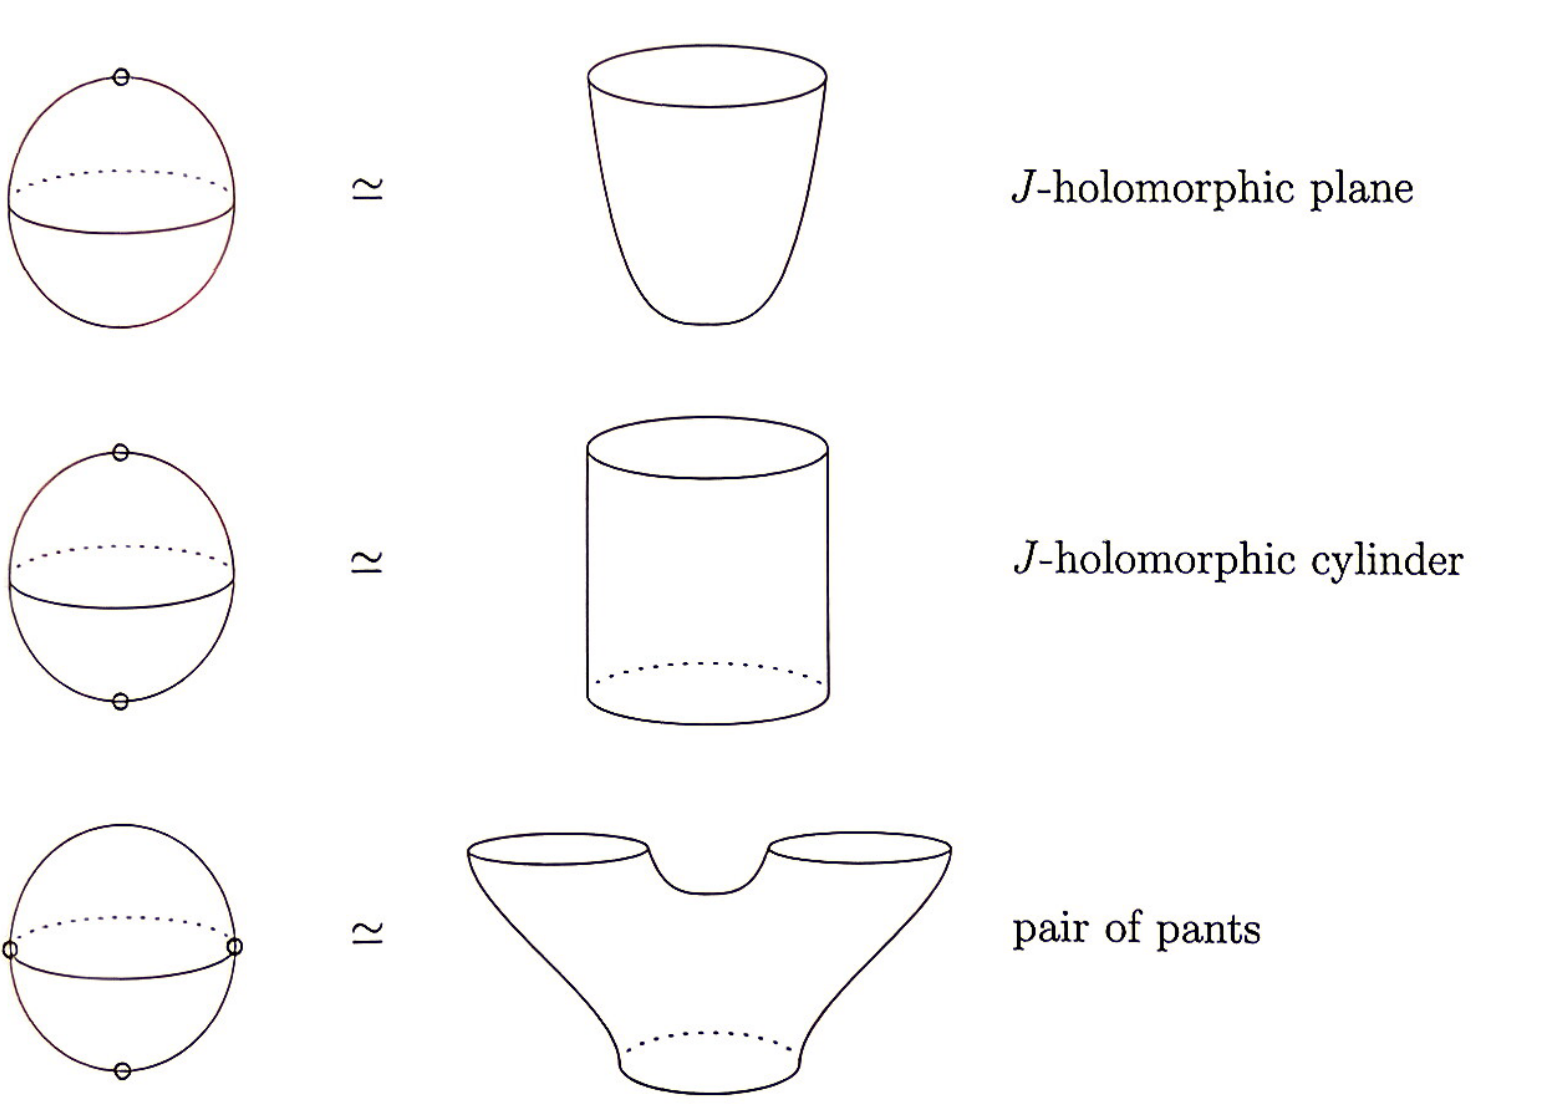
\includegraphics[width=0.72\linewidth]{figures/fig_p074_2.png}
  \caption*{图 3.7\quad $S^2$ 上不同数目的刺点
  （原书 p.66, Figure 3.7）}
\end{figure}

经过上面引入的刺点修改，$u:(\dot\Sigma,j)\to(SM,\dd(\ee^r\alpha),J)$ 才可能
作为 $J$-全纯曲线而良定义。例如，对 $S^2\setminus\{(1,0,0)\}$（其中
$(1,0,0)$ 表示 $S^2$ 的北极），在刺点上施加双全纯映射之后，它可以作为
$J$-全纯曲线嵌入 $SM$，但要小心选取刺点 $(1,0,0)$ 的「开口方向」
（见图 3.8）。

% >>> p075
\begin{figure}[htbp]
  \centering
  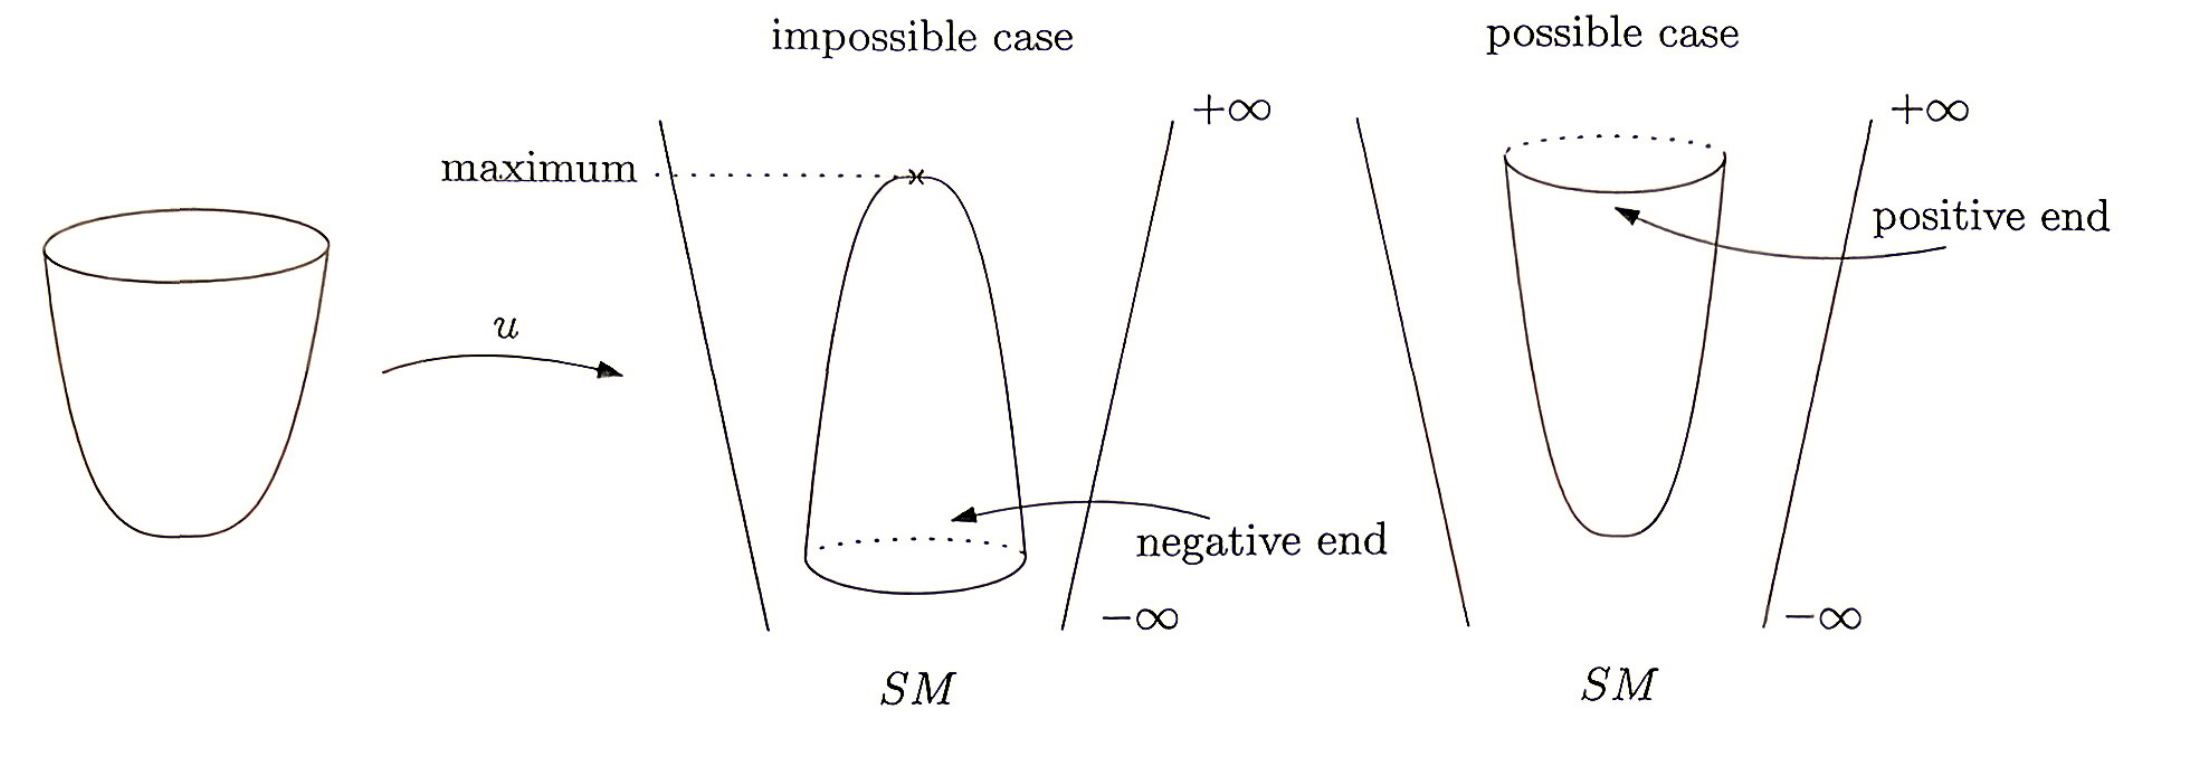
\includegraphics[width=0.82\linewidth]{figures/fig_p075_1.png}
  \caption*{图 3.8\quad 把带刺点的 $S^2$ 作为 $J$-全纯曲线嵌入 $SM$
  （原书 p.67, Figure 3.8）}
\end{figure}

在第一种选择下，$(S^2\setminus\{(1,0,0)\},j)$ 的像带有\textbf{负柱端}
（negative cylindrical end）；而在第二种选择下，
$(S^2\setminus\{(1,0,0)\},j)$ 的像带有\textbf{正柱端}
（positive cylindrical end）。由于 $\R$ 分量函数是次调和的，第一种选择被
排除。一般地，我们得到如下有用的命题：

\begin{wprop}{3.3.1}
任何非常值的 $J$-全纯曲线
$u:(\dot\Sigma,j)\to(SM,\dd(\ee^r\alpha),J)$ 必至少有一个正端。
\end{wprop}

% [Tutor Note: 含糊点拨——命题 3.3.1 的证明要点正是上面的极大值原理：若曲线
% 只有负端，则在 $s\to-\infty$ 处 $u_\R\to-\infty$，而在紧的「中部」$u_\R$
% 取到最大值，与次调和函数的极大值原理矛盾。这里需要 $J$-全纯曲线在刺点附近
% 的渐近行为（定理 3.3.1）来保证端的存在与符号；教材把它留作显然，实际用到
% 了 Hofer 的渐近分析（[120]）。]

接下来考虑 $(\dot\Sigma_{g=0}=S^2\setminus\{p_1,p_2\},j)$。按例 3.3.1 中的
双全纯映射（在同痕意义下），把它等同于柱面 $\R\times S^1$。下面是与问题 3
相关的一个例子。

\begin{wexam}{3.3.2}
给定带闭 Reeb 轨道 $\gamma(t)$（周期 $T>0$）的切触流形 $(M,\alpha)$，考虑
映射 $u_{\mathrm{trivial}}:\R\times S^1\to\R\times M$，定义为
\begin{equation}\tag{3.22}
  u_{\mathrm{trivial}}(s,t):=(Ts,\gamma(Tt))
  =:(u_\R,u_M).
\end{equation}
可以验证 $u_\R$ 与 $u_M$ 满足如下方程：
\[
  \frac{\partial u_\R}{\partial s}
  -\alpha\Bigl(\frac{\partial u_M}{\partial t}\Bigr)
  =T-T\cdot\alpha\bigl(R_\alpha(\gamma(Tt))\bigr)=0,
\]
以及
\[
  J\pi_\xi\Bigl(\frac{\partial u_M}{\partial t}\Bigr)
  +\pi_\xi\Bigl(\frac{\partial u_M}{\partial s}\Bigr)
  =J\pi_\xi\bigl(T\cdot R_\alpha(\gamma(Tt))\bigr)=0 .
\]
因此，(3.19) 与 (3.20) 表明 $u_{\mathrm{trivial}}$ 确实是 $J$-全纯曲线。
由于 $u_M$ 不依赖于 $s$，且对每个 $s\in\R$，$M$ 分量都是同一条由闭 Reeb
轨道 $\gamma(Tt)$ 给出的圆周，$u_{\mathrm{trivial}}$ 之名由此得其实：它是一条
\textbf{平凡的 $J$-全纯柱面}（见图 3.9）。

那么 $u_{\mathrm{trivial}}$ 的能量 $E(u_{\mathrm{trivial}})$ 如何？回忆由
(1.9)，$J$-全纯曲线 $u:(\Sigma,j)\to(M,\omega)$ 的能量定义为
$\int_\Sigma u^*\omega$。若把此定义直接用于 $u_{\mathrm{trivial}}$，计算如下

% >>> p076
\begin{figure}[htbp]
  \centering
  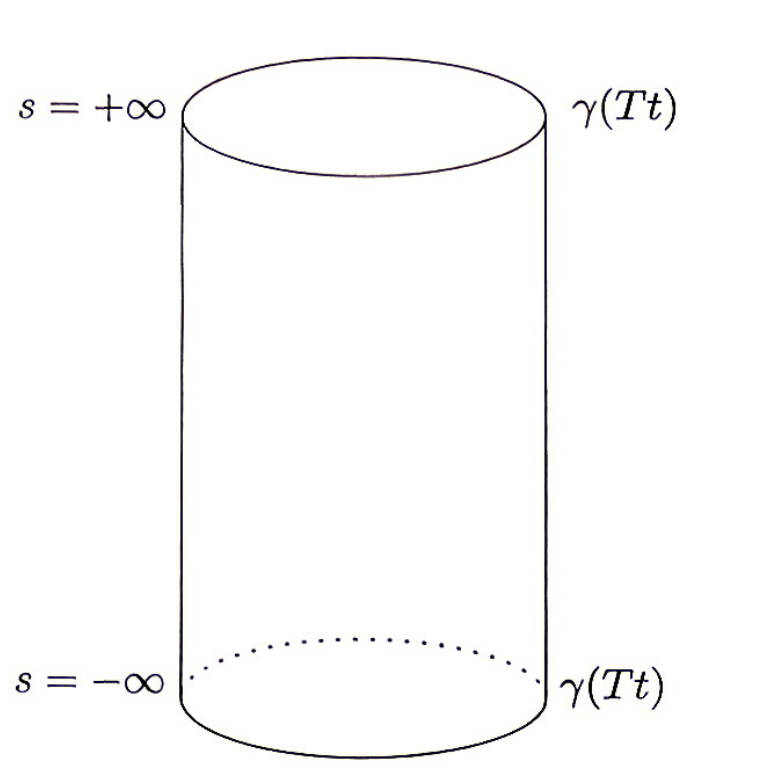
\includegraphics[width=0.42\linewidth]{figures/fig_p076_1.png}
  \caption*{图 3.9\quad 一条平凡的 $J$-全纯柱面
  （原书 p.68, Figure 3.9）}
\end{figure}

\begin{equation}\tag{3.23}
\begin{aligned}
  E(u_{\mathrm{trivial}})
  &=\int_{\R\times S^1}u_{\mathrm{trivial}}^*\dd(\ee^r\alpha)\\
  &=\int_{-\infty}^{\infty}\int_0^1
   \ee^{Ts}(\dd r\wedge\alpha+\dd\alpha)
   \Bigl(\frac{\partial u}{\partial s},\frac{\partial u}{\partial t}\Bigr)
   \,\dd s\,\dd t\\
  &=\int_{-\infty}^{\infty}\int_0^1
   \ee^{Ts}(\dd r\wedge\alpha+\dd\alpha)
   \bigl((T,0),(0,TR_\alpha)\bigr)\,\dd s\,\dd t\\
  &=T^2\int_{-\infty}^{\infty}\ee^{Ts}\,\dd s=+\infty .
\end{aligned}
\end{equation}
(3.23) 的计算结果令人不安：即使曲线在某种意义上平凡，我们也无法从
$E(u_{\mathrm{trivial}})$ 读出任何有用的信息。\hfill$//$
\end{wexam}

在其重要论文 [120] 中，H. Hofer 想出一个巧妙办法来修正这一「平凡曲线却具有
无穷能量」的问题：考虑函数 $\varphi=\frac{2}{\pi}\arctan x$ 以及形变辛结构
$\omega_\varphi:=\dd(\ee^{\varphi(r)}\alpha)$。容易验证 $J$ 也与
$\omega_\varphi$ 相容。此时，能量 $E_\varphi$（关于 $\omega_\varphi$）可如下
定义并计算：
\begin{align*}
  E_\varphi(u_{\mathrm{trivial}})
  &:=\int_{\R\times S^1}u_{\mathrm{trivial}}^*\omega_\varphi\\
  &=\int_{-\infty}^{\infty}\int_0^1\ee^{\varphi(Ts)}
   \bigl(\varphi'(Ts)\dd r\wedge\alpha+\dd\alpha\bigr)
   \bigl((T,0),(0,TR_\alpha)\bigr)\,\dd s\,\dd t\\
  &=\int_{-\infty}^{\infty}\int_0^1
   \ee^{\varphi(Ts)}\varphi'(Ts)\cdot T^2\,\dd s\,\dd t\\
  &=T^2\int_{-\infty}^{\infty}\ee^{\varphi(Ts)}\varphi'(Ts)\,\dd s\\
  &=T\int_{-\infty}^{\infty}\ee^{\varphi(A)}\varphi'(A)\,\dd A
   =T\int_{-1}^{1}\ee^B\,\dd B<+\infty,
\end{align*}
其中作了变量替换 $A=Ts$、$B=\varphi(A)$。

% [Tutor Note: 原文疑误——定义 3.3.1 的 (3.25) 中写作
% 「$\varphi(t)\to\pm\infty$（$t\to\pm\infty$）」，但按定义 3.3.1 正文
% $\varphi:\R\to(-1,1)$ 的取值以及上一段
% $\varphi=\frac{2}{\pi}\arctan x$（其极限为 $\pm1$），此处应为
% $\varphi(t)\to\pm1$。只有极限为 $\pm1$ 时，上面的末行
% $\int_{-1}^{1}\ee^B\,\dd B$ 才成立。已记入 review_ch03.md。]

% >>> p077
一般地，可给出如下定义。

\begin{wdefn}{3.3.1}（Hofer 能量 [120]）
设 $(M,\xi=\ker\alpha)$ 是切触流形，$SM$ 表示其辛化。对任意 $J$-全纯曲线
$u:(\dot\Sigma,j)\to(SM,\dd(\ee^r\alpha),J)$，\textbf{$u$ 的 Hofer 能量}
$E_{\mathrm{Hofer}}(u)$ 定义如下：
\begin{equation}\tag{3.24}
  E_{\mathrm{Hofer}}(u)
  :=\sup\Bigl\{\int_{\dot\Sigma}u^*\bigl(\dd(\ee^{\varphi(r)}\alpha)\bigr)
  \ \Big|\ \varphi\ \text{满足下面的条件 (3.25)}\Bigr\},
\end{equation}
其中函数 $\varphi:\R\to(-1,1)$ 满足
\begin{equation}\tag{3.25}
  \varphi(0)=0,\qquad \varphi'>0,\qquad
  \varphi(t)\to\pm1\quad(t\to\pm\infty).
\end{equation}
\end{wdefn}

这一定义的重要性体现在下述基本定理中，它开启了把（带刺点的）$J$-全纯曲线
作为研究 Reeb 动力学之有效方法的门户。

\begin{wthm}{3.3.1}（[120] 中定理 31）
设 $(M,\xi=\ker\alpha)$ 是切触流形，$SM$ 表示其辛化。假设
$u:(\dot\Sigma,j)\to(SM,\dd(\ee^r\alpha),J)$ 是满足
$E_{\mathrm{Hofer}}(u)<+\infty$ 的 $J$-全纯曲线。则在每个刺点 $\Gamma$
附近，经由映射 (3.21) 的等同下，有
\[
  \lim_{s\to\pm\infty}u(s,\cdot)=\gamma(T\,\cdot),
\]
其中 $\gamma$ 是 $(M,\xi=\ker\alpha)$ 的周期为 $T$ 的闭 Reeb 轨道。
\end{wthm}

% [Tutor Note: 原文疑误——定理 3.3.1 中把曲线定义域写作
% $u:(\dot\Sigma\setminus\Gamma,j)$，但按本节记号
% $\dot\Sigma=\Sigma\setminus\Gamma$ 已含刺点集，再减去 $\Gamma$ 是重复的；
% 应为 $u:(\dot\Sigma,j)$。已记入 review_ch03.md。]

作为 $u$ 之极限的那些闭 Reeb 轨道 $\gamma$，称为 $u$ 的\textbf{渐近端}
（asymptotic ends）。对 $s\to\infty$，相应的 $\gamma$ 称为 $u$ 的
\textbf{正（渐近）轨道}；对 $s\to-\infty$，相应的 $\gamma$ 称为
\textbf{负（渐近）轨道}。示意图见图 3.10，其中 $u$ 有两条正轨道与一条负轨道。

\begin{figure}[htbp]
  \centering
  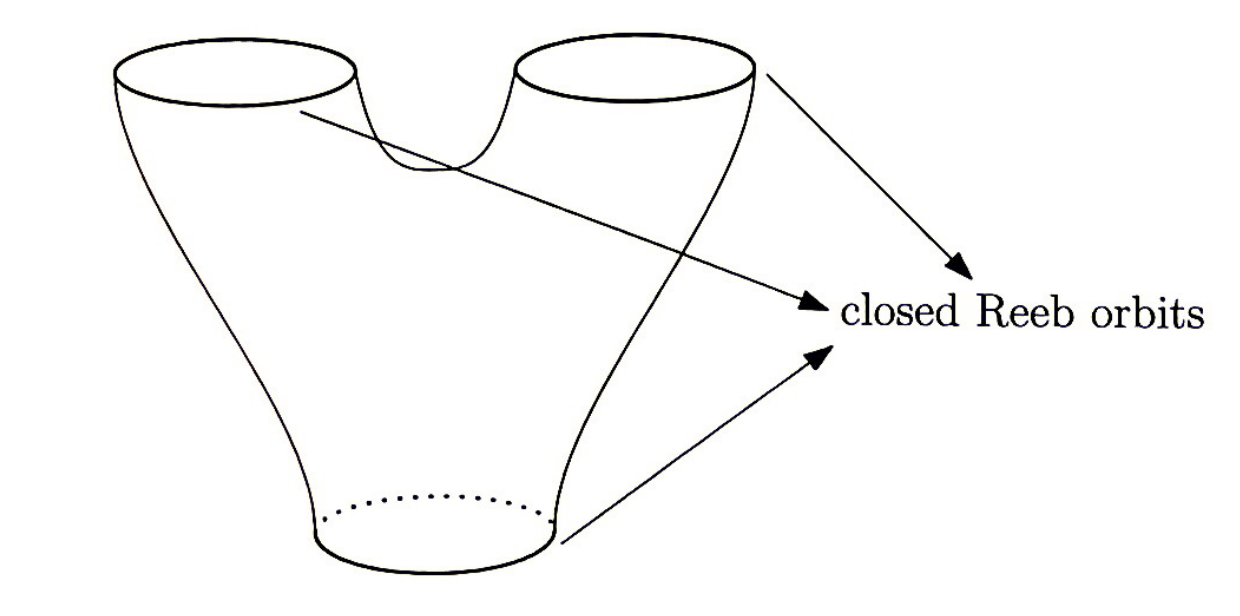
\includegraphics[width=0.62\linewidth]{figures/fig_p077_1.png}
  \caption*{图 3.10\quad 端附近的闭 Reeb 轨道
  （原书 p.69, Figure 3.10）}
\end{figure}

\begin{wrem}{3.3.1}
回忆 Weinstein 猜想（猜想 3.1.1）断言闭 Reeb 轨道的存在性。人们或许会想
直接应用定理 3.3.1 来迅速断定猜想 3.1.1 成立（其中 $\gamma$ 由某条
$J$-全纯曲线的渐近轨道给出）。
\end{wrem}

% >>> p078
然而这里有一个本质的缺口——我们如何知道这样的 $J$-全纯曲线存在？事实证明，
证明（具有指定渐近轨道的）$J$-全纯曲线的存在性，是辛几何中最困难、最核心的
问题之一，通常要用模空间方法来研究（参看第 8 章 §8.3）。
